\documentclass[12pt,a4paper]{article}
\usepackage[utf8]{inputenc}
\usepackage[spanish]{babel}
\usepackage{amsmath}
\usepackage{amsfonts}
\usepackage{amssymb}
\usepackage{graphicx}
\usepackage[left=2.5cm,right=2.5cm,top=3cm,bottom=3cm]{geometry}
\usepackage{xcolor}
\usepackage{listings}
\usepackage{tcolorbox}
\usepackage{hyperref}

% Configuración de colores para código
\definecolor{codegreen}{rgb}{0,0.6,0}
\definecolor{codegray}{rgb}{0.5,0.5,0.5}
\definecolor{codepurple}{rgb}{0.58,0,0.82}
\definecolor{backcolour}{rgb}{0.95,0.95,0.92}

\lstdefinestyle{mystyle}{
    backgroundcolor=\color{backcolour},   
    commentstyle=\color{codegreen},
    keywordstyle=\color{magenta},
    numberstyle=\tiny\color{codegray},
    stringstyle=\color{codepurple},
    basicstyle=\ttfamily\footnotesize,
    breakatwhitespace=false,         
    breaklines=true,                 
    captionpos=b,                    
    keepspaces=true,                 
    numbers=left,                    
    numbersep=5pt,                  
    showspaces=false,                
    showstringspaces=false,
    showtabs=false,                  
    tabsize=2
}
\lstset{style=mystyle}

\title{\textbf{Manual de Proyectos de Laboratorio}\\ \Large Física y Sistemas Embebidos}
\author{Andrés}
\date{\today}

\begin{document}

\maketitle
\tableofcontents
\newpage

\section{Proyecto 1: Servidor Web IoT con ESP32}
\subsection{Introducción}
En este proyecto se transforma un ESP32 en un poderoso Servidor Web Local para el Internet de las Cosas (IoT). Se vincula el mundo físico con el digital: usando un potenciómetro real para recopilar datos de voltaje y verlos graficados profesionalmente (con Google Charts y Plotly) en tiempo real en el navegador. Al mismo tiempo, se controla un LED físico de forma inalámbrica mediante una red Wi-Fi.

\subsection{Materiales y Ensamblaje del Circuito}
\begin{itemize}
    \item Placa ESP32 (DOIT ESP32 DEVKIT V1)
    \item Potenciómetro de $10\text{k}\Omega$
    \item LED y Resistencia ($220\Omega - 330\Omega$)
    \item Protoboard y Jumpers
\end{itemize}

\begin{tcolorbox}[colback=blue!5!white,colframe=blue!75!black,title=Detalle de Pines]
\textbf{Potenciómetro:} GND, GPIO34 (Señal), 3.3V.\\
\textbf{LED:} GPIO4 al Ánodo (mediante resistencia); GND al Cátodo.
\end{tcolorbox}

\begin{figure}[h]
    \centering
    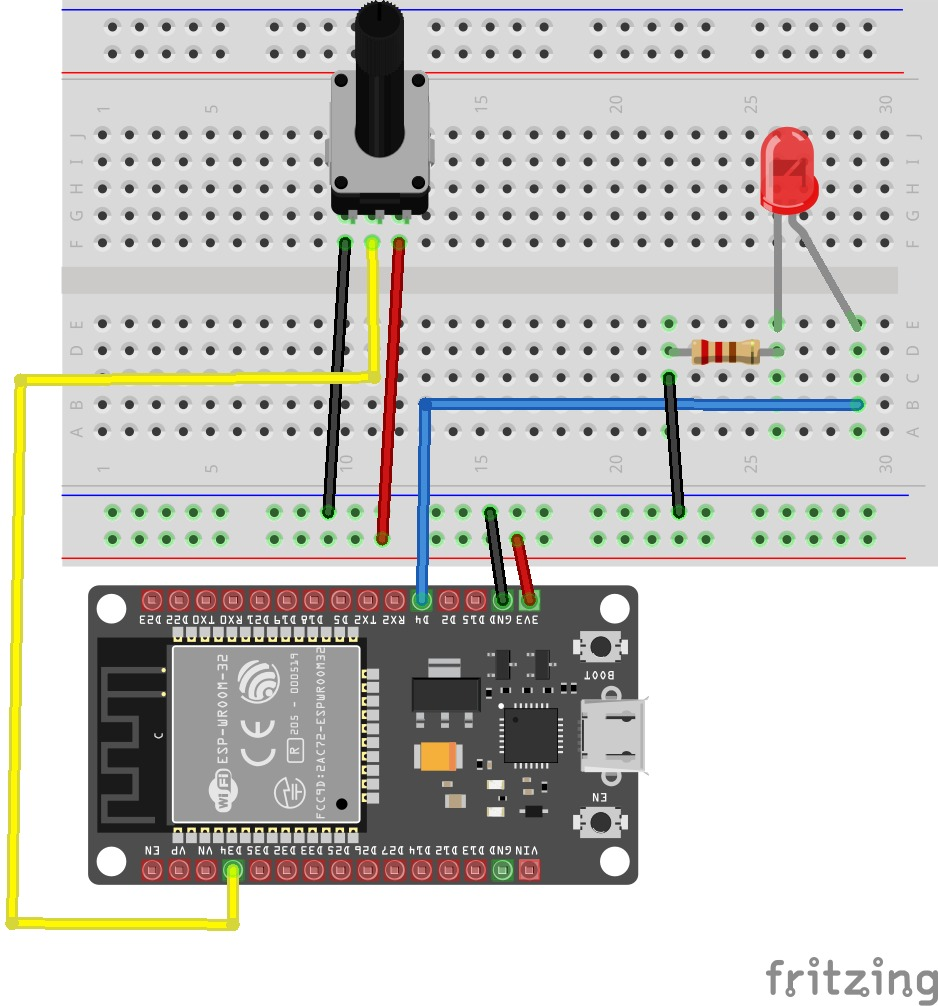
\includegraphics[width=0.7\textwidth]{circuito.jpeg}
    \caption{Diagrama de conexiones en la protoboard.}
\end{figure}

\subsection{Código Fuente}
A continuación, se presenta el código principal para el ESP32 usando el IDE de Arduino.

\begin{lstlisting}[language=C++]
#include <WiFi.h>
#include <WebServer.h>

const char* miSSID     = "Andres";       
const char* miPASSWORD = "andres10";     

const int pinPotenciometro = 34; 
const int pinLED = 4;            

bool ledEncendido = false;
WebServer servidor(80);

void setup() {
  Serial.begin(115200);
  pinMode(pinLED, OUTPUT);
  digitalWrite(pinLED, LOW);

  WiFi.begin(miSSID, miPASSWORD);
  while (WiFi.status() != WL_CONNECTED) { 
      delay(500); 
      Serial.print("."); 
  }
  
  // (El codigo HTML se ha omitido por brevedad en este documento)
  servidor.on("/datos", []() {
    float v = (analogRead(pinPotenciometro) * 3.3) / 4095.0;
    servidor.send(200, "application/json", "{\"voltaje\": " + String(v, 2) + "}");
  });
  
  servidor.on("/led", []() {
    ledEncendido = !ledEncendido;
    digitalWrite(pinLED, ledEncendido ? HIGH : LOW);
    servidor.send(200, "text/plain", "OK");
  });

  servidor.begin();
}

void loop() { 
    servidor.handleClient(); 
}
\end{lstlisting}

\newpage

\section{Proyecto 2: Detector de Temperatura con Pantalla y Alarma}
\subsection{Introducción}
En este proyecto se construye un termómetro digital inteligente utilizando Arduino. El sistema interactúa con un sensor de temperatura y humedad (DHT11), muestra los datos en tiempo real en una pantalla LCD I2C y programa una lógica de control que enciende un LED de advertencia cuando la temperatura supera los $28^\circ\text{C}$.

\subsection{Materiales y Ensamblaje del Circuito}
\begin{itemize}
    \item Placa Arduino Uno (o equivalente)
    \item Sensor de Temperatura y Humedad DHT11
    \item Pantalla LCD 16x2 con Módulo I2C
    \item LED rojo y Resistencia ($220\Omega - 330\Omega$)
    \item Protoboard y Jumpers
\end{itemize}

\begin{tcolorbox}[colback=red!5!white,colframe=red!75!black,title=Detalle de Pines]
\textbf{Sensor DHT11:} VCC a 5V, GND a GND, Señal al Pin Digital 2.\\
\textbf{Pantalla LCD I2C:} VCC a 5V, GND a GND, SDA al pin A4, SCL al pin A5.\\
\textbf{LED de Alarma:} Pin Digital 8 al Ánodo (mediante resistencia); GND al Cátodo.
\end{tcolorbox}

\begin{figure}[h]
    \centering
    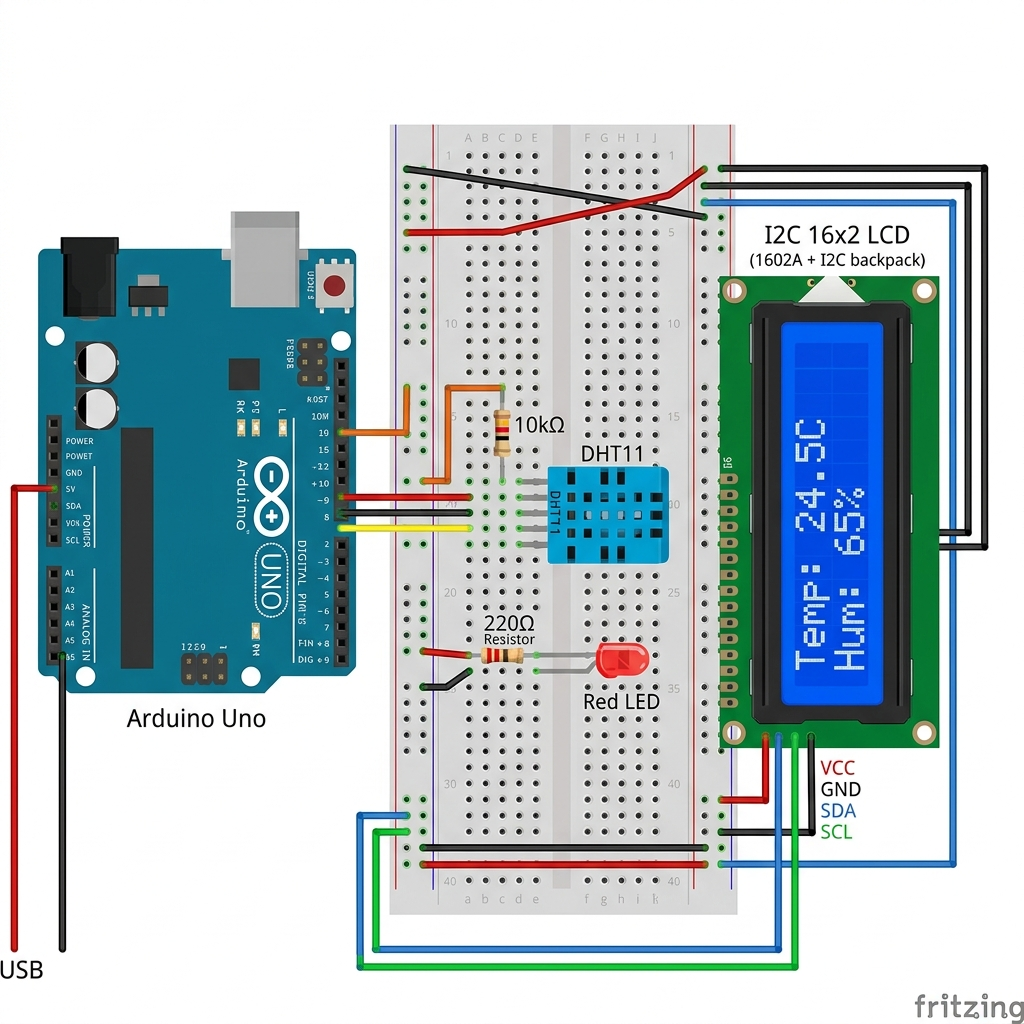
\includegraphics[width=0.7\textwidth]{circuito_temperatura.png}
    \caption{Diagrama del circuito del detector de temperatura.}
\end{figure}

\subsection{Código Fuente}
\begin{lstlisting}[language=C++]
#include <Wire.h>
#include <LiquidCrystal_I2C.h>
#include <DHT.h>

#define DHTPIN 2       
#define DHTTYPE DHT11  
DHT dht(DHTPIN, DHTTYPE);

LiquidCrystal_I2C lcd(0x27, 16, 2);

const int pinLedAlarma = 8;
const float LIMITE_TEMPERATURA = 28.0; 

void setup() {
  Serial.begin(9600);
  pinMode(pinLedAlarma, OUTPUT);
  digitalWrite(pinLedAlarma, LOW);

  dht.begin();
  lcd.init();
  lcd.backlight();
  lcd.setCursor(0, 0);
  lcd.print("Iniciando...");
  delay(2000);
  lcd.clear();
}

void loop() {
  delay(2000);
  float h = dht.readHumidity();
  float t = dht.readTemperature();

  if (isnan(h) || isnan(t)) {
    lcd.setCursor(0, 0);
    lcd.print("Error de sensor!");
    return;
  }

  lcd.setCursor(0, 0);
  lcd.print("Temp: "); lcd.print(t, 1); lcd.print(" C   ");

  lcd.setCursor(0, 1);
  lcd.print("Hum:  "); lcd.print(h, 1); lcd.print(" %   ");

  if (t > LIMITE_TEMPERATURA) {
    digitalWrite(pinLedAlarma, HIGH);
  } else {
    digitalWrite(pinLedAlarma, LOW);
  }
}
\end{lstlisting}

\newpage

\section{Proyecto 3: Laboratorio Virtual - Doppler Nexus}
\subsection{Introducción}
Este proyecto es una simulación interactiva avanzada (programada en Vanilla JS y HTML5 Canvas) que permite explorar el Efecto Doppler en 2D. Se demuestra visualmente cómo el movimiento relativo entre una fuente sonora y un observador afecta la frecuencia percibida. Además, simula el fenómeno de la ruptura de la barrera del sonido y la formación del Cono de Mach.

\subsection{Características del Laboratorio}
\begin{itemize}
    \item \textbf{Renderizado en tiempo real:} Emisión continua de frentes de onda (círculos concéntricos) que se expanden a la velocidad del sonido simulada.
    \item \textbf{Aceleración Espacial:} Control dinámico de la velocidad de la fuente sonora en relación a la velocidad de la onda ($v_s / v$).
    \item \textbf{Explosión Sónica (Sonic Boom):} Visualización matemática de la envolvente cónica cuando $v_s > v$.
\end{itemize}

\begin{tcolorbox}[colback=purple!5!white,colframe=purple!75!black,title=Fórmulas Implementadas]
\textbf{Observador en movimiento:} 
\[ f' = f \left( \frac{v \pm v_o}{v} \right) \]
\textbf{Fuente en movimiento:}
\[ f' = f \left( \frac{v}{v \mp v_s} \right) \]
Donde $v$ es la velocidad de la onda, $v_o$ la velocidad del observador, y $v_s$ la velocidad de la fuente.
\end{tcolorbox}

\subsection{Lógica Principal de Animación}
En la implementación, cada frente de onda es un objeto independiente en un arreglo, cuya posición central corresponde a la posición de la fuente en el instante de emisión.
\begin{lstlisting}[language=JavaScript]
// Ciclo de animacion (requestAnimationFrame)
function animar() {
    ctx.clearRect(0, 0, canvas.width, canvas.height);
    
    // Actualizar posicion de la fuente
    fuente.x += fuente.vx;
    
    // Emitir nueva onda cada 'T' frames
    if (frames % T === 0) {
        ondas.push({ x: fuente.x, y: fuente.y, radio: 0 });
    }
    
    // Dibujar y expandir ondas
    ondas.forEach(onda => {
        onda.radio += v_sonido; // Expandir a velocidad constante
        ctx.beginPath();
        ctx.arc(onda.x, onda.y, onda.radio, 0, Math.PI * 2);
        ctx.stroke();
    });
    
    frames++;
    requestAnimationFrame(animar);
}
\end{lstlisting}

\end{document}
